
% --------------------------------
% 
% --------------------------------

\section{Mexico City Prospective Study (MCPS)}

% --------------------------------
% Recruitment and baseline data
% --------------------------------
\subsection{Recruitment and baseline data}
\begin{frame}
    \frametitle{Recruitment and baseline data}
    \framesubtitle{Overview}

    \begin{columns}

    % Text
    \begin{column}{0.5\textwidth}

        \begin{figure}[htpb]
            \centering
            
\includegraphics[width=1.15\textwidth]{ziyatdinov2023/tapia-conyer2006_header.png}
        \end{figure}

        Over \textbf{\color{complement-1} 150,000} participants were recruited in two districts (figure \ref{fig:mcps-main-map}) between \textbf{\color{complement-2} 1998 and 2004}.

        \begin{itemize}[label=$\bullet$,noitemsep,topsep=5pt]
            \item Baseline questionnaire.
            \item Blood samples.
            \item Physical measurements.
            \item Linkage to mortality.
        \end{itemize}

    \end{column}

    % Image
    \begin{column}{0.5\textwidth}
        \begin{figure}[htpb]
            \centering
            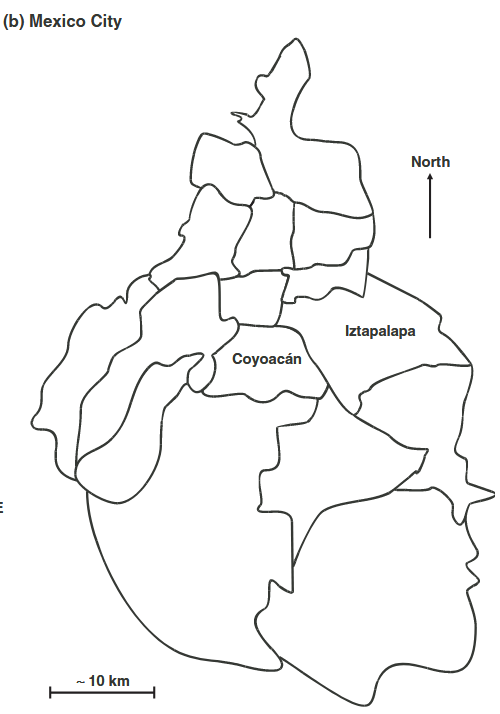
\includegraphics[width=0.45\textwidth]{ziyatdinov2023/map.png}
            \caption{Map showing the location of the MCPS districts \parencite{tapia-conyer-2006}.}
            \label{fig:mcps-main-map}
        \end{figure}
    \end{column}
    \end{columns}
\end{frame}


\begin{frame}
    \frametitle{Recruitment and baseline data}
    \framesubtitle{Baseline data and samples}
    
    \begin{columns}
    % Column 1
    \begin{column}{0.33\textwidth}

        \begin{itemize}[itemsep=2.5pt,topsep=0pt]
            \item \textbf{\color{primary-color} Socio-demographic}
            \begin{itemize}[label=$\bullet$,noitemsep,topsep=1pt]
                {\small\color{complement-text}
                    \item Age and sex
                    \item Area of residence
                    \item Marital status
                    \item Educational achievement
                    \item Occupation
                    \item Income
                    \item Health service provider
                }
            \end{itemize}
            \item \textbf{\color{primary-color} Lifestyle characteristics}
            \begin{itemize}[label=$\bullet$,noitemsep,topsep=1pt]
                {\small\color{complement-text}
                    \item Diet (fruit/vegetables, fried food, types of oil)
                    \item Smoking and alcohol
                    \item Physical activity
                    \item Sleep duration
                }
            \end{itemize}
            \item \textbf{\color{primary-color} Prior diseases and medications}
        \end{itemize}

    \end{column}
    
    % Column 2
    \begin{column}{0.33\textwidth}
        \begin{itemize}[itemsep=2.5pt,topsep=0pt]
            \item \textbf{\color{primary-color} Reproductive history (women)}
            \begin{itemize}[label=$\bullet$,noitemsep,topsep=1pt]
                {\small\color{complement-text}
                    \item Menopausal status
                    \item Hysteroctomy
                    \item Oopheroctomy
                    \item HRT
                    \item Contraceptive use
                    \item Pregnancy (age and number)
                }
            \end{itemize}
            \item \textbf{\color{primary-color} Physical measurements}
            \begin{itemize}[label=$\bullet$,noitemsep,topsep=1pt]
                {\small\color{complement-text}
                    \item Height
                    \item Weight
                    \item Waist and hip circumferece
                    \item Systolic and diastolic blood pressure
                }
            \end{itemize}
        \end{itemize}
    \end{column}

    % Column 3
    \begin{column}{0.33\textwidth}
        \begin{itemize}[itemsep=2.5pt,topsep=0pt]
            \item \textbf{\color{primary-color} Blood samples}
            \begin{itemize}[label=$\bullet$,noitemsep,topsep=1pt]
                {\small\color{complement-text}
                    \item Plasma \& buffy coat
                    \item HbA1c and other essays
                    \item NMR metabolomics
                }
            \end{itemize}
        \end{itemize}
    \end{column}
    
    \end{columns}

\end{frame}

% --------------------------------
% Genetic overview
% --------------------------------
\subsection{Genetic overview}
\begin{frame}
    \frametitle{Genetic overview}
    \framesubtitle{Genetic datasets}

    \begin{columns}
    % Column 1
    \begin{column}{0.5\textwidth}

        Genetic datasets were added later \parencite{ziyatdinov2023}, making it one of the \textbf{\color{complement-1} largest} studies for \textit{non-eurpean} populations.

        \begin{itemize}[itemsep=2pt,topsep=10pt]
            \item<1-> \textbf{\color{primary-color} Genome-Wide Genotyping}
            \begin{itemize}[label=$\bullet$,noitemsep,topsep=0pt]
                \item Illumina - GSAv2 chip array
                \item $n =$ 138,511 individuals
            \end{itemize}
            \item<2-> \textbf{\color{primary-color} Exome Sequencing (WES)}
            \begin{itemize}[label=$\bullet$,noitemsep,topsep=0pt]
                \item $n =$ 141,046 individuals
            \end{itemize}
            \item<3-> \textbf{\color{primary-color} Whole-Genome Sequencing (WGS)}
            \begin{itemize}[label=$\bullet$,noitemsep,topsep=0pt]
                \item $n =$ 9,950 individuals
            \end{itemize}
        \end{itemize}
    \end{column}
    
    % Column 2
    \begin{column}{0.5\textwidth}
        \begin{figure}[htpb]
            \centering
            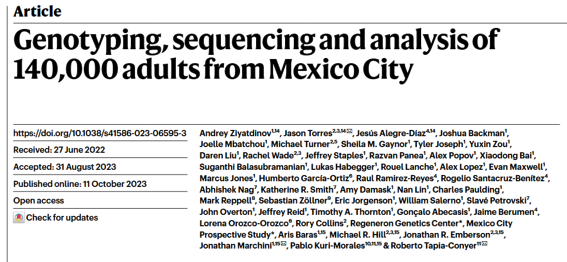
\includegraphics[width=\textwidth]{ziyatdinov2023/ziyatdinov2023_header.png}
        \end{figure}
    \end{column}
    \end{columns}
\end{frame}

% -------------------------
% Family networks
% -------------------------
\subsection{Family networks}
\begin{frame}
    \frametitle{Family networks}
    \framesubtitle{IBD estimates}

    \begin{columns}
        % Column 1
        \begin{column}{0.5\textwidth}

            At least \textbf{\color{primary-color} 71\% of the population} has a relative present in the dataset.

            \begin{itemize}[label=$\bullet$,noitemsep,topsep=5pt]
                \item \textbf{Parent-offspring:} 31,597 relationships
                \item \textbf{Sibling pairs:} 31,597 relationships
            \end{itemize}

            Close relatedness is explained by families living in \textbf{close proximity}.

            \begin{equation}
              x = 2 \times y
            \end{equation}

        \end{column}
        % Column 2
        \begin{column}{0.5\textwidth}
            \begin{figure}[htpb]
                \centering
                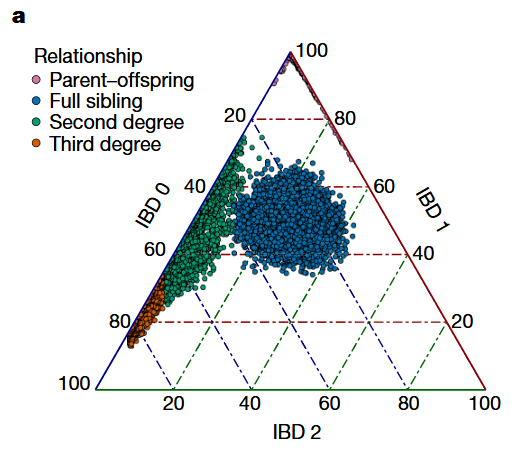
\includegraphics[width=0.85\textwidth]{ziyatdinov2023/familial-relatedness-a.png}
                \caption{Percentage of genome-estimated to have 0 to 3 IBD alleles \parencite{ziyatdinov2023}.}
                \label{fig:percent-genome-ibd}
            \end{figure}
        \end{column}
    \end{columns}

\end{frame}

% Comparison of family networks
\begin{frame}
    \frametitle{Main findings}
    \framesubtitle{Dataset comparisons}

    % Please add the following required packages to your document preamble:
    % \usepackage{booktabs}
    % \usepackage[table,xcdraw]{xcolor}
    % Beamer presentation requires \usepackage{colortbl} instead of \usepackage[table,xcdraw]{xcolor}
    \begin{table}[]
    \caption{Comparison of family network sizes in MCPS, GHS and UKB datasets \parencite{ziyatdinov2023}.}
    \begin{tabular}{@{}cccc@{}}
    \toprule
    %\rowcolor{primary-color} 
    \textbf{}                                  & \textbf{MCPS   150k} & \textbf{GHS   145k} & \textbf{UKB   450k} \\ \midrule
    Parent-child relationships                 & 31,597 (33.1\%)      & 29,599 (31.1\%)     & 6,270 (2.3\%)       \\
    Full-sibling relationships                 & 29,482 (26.9\%)      & 18,540 (18.9\%)     & 22,657 (8.5\%)      \\
    2nd-degree relationships                   & 47,080 (31.2\%)      & 71,766 (42.4\%)     & 11,169 (4.2\%)      \\
    3rd-degree relationships                   & 120,180 (45.2\%)     & 129,782 (48.0\%)    & 66,847 (19.8\%)     \\
    Number of pedigrees                        & 22,766               & 19,770              & 24,560              \\
    Pedigrees with \textgreater{}2 individuals & 9,889                & 7,998               & 2590                \\
    Individuals with both parents (trios)      & 5,603                & 5,448               & 1,065               \\
    Pedigrees \textgreater{}2 generations      & 600                  & 2,299               & 0                   \\ \bottomrule
    \end{tabular}
    \label{tab:comparison-families}
    \end{table}
\end{frame}